\documentclass[svgnames,11pt]{beamer}
\input{/home/tof/Documents/Cozy/latex-include/preambule_commun.tex}
\input{/home/tof/Documents/Cozy/latex-include/preambule_beamer.tex}
%\usepackage{pgfpages} \setbeameroption{show notes on second screen=left}
\author[]{Christophe Viroulaud}
\title{Listes chaînées}
\date{\framebox{\textbf{Archi 03}}}
%\logo{}
\institute{Terminale - NSI}

\begin{document}
\begin{frame}
    \titlepage
\end{frame}
\begin{frame}
    \frametitle{}

    Quand un tableau est créé, le système lui alloue un espace contigu en mémoire.
    \begin{center}
        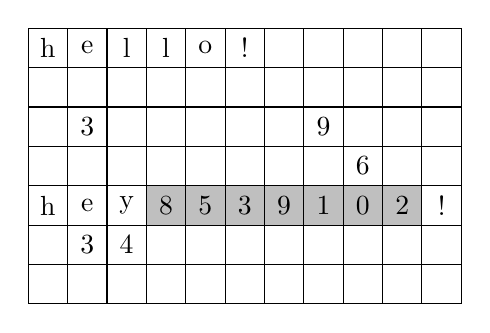
\begin{tikzpicture}[scale=0.5]
            \fill[gray!50] (3,2) rectangle (10,3);
            \draw (0,0) grid (11,7);

            \draw (0.5,2.5) node{h};
            \draw (1.5,2.5) node{e};
            \draw (2.5,2.5) node{y};

            \draw (0.5,6.5) node{h};
            \draw (1.5,6.5) node{e};
            \draw (2.5,6.5) node{l};
            \draw (3.5,6.5) node{l};
            \draw (4.5,6.5) node{o};
            \draw (5.5,6.5) node{!};

            \draw (10.5,2.5) node{!};
            \draw (7.5,4.5) node{9};
            \draw (8.5,3.5) node{6};
            \draw (1.5,4.5) node{3};
            \draw (2.5,1.5) node{4};
            \draw (1.5,1.5) node{3};

            \foreach \x/\y in {3/8,4/5,5/3,6/9,7/1,8/0,9/2}
                {\draw (\x+0.5,2.5) node{\y};}
        \end{tikzpicture}
        \captionof{figure}{Le tableau est enregistré dans un espace libre}
        \label{IMG}
    \end{center}
    On accède à chaque élément du tableau \textbf{en temps constant}. Cependant insérer un nouvel élément devient problématique.
    \note{vrai en C, un peu différent en Python (haut-niveau)}

\end{frame}
\begin{frame}
    \frametitle{}

    \begin{framed}
        Comment définir un autre type de structure de données qui pallie les limitations d'un tableau?
    \end{framed}

\end{frame}
\section{Liste chaînée}
\subsection{Principe}
\begin{frame}
    \frametitle{Liste chaînée - principe}
    Chaque élément:
    \begin{itemize}
        \item<1-> prend une place libre quelconque en mémoire.
        \item<2-> connaît l'emplacement de l'élément suivant.
    \end{itemize}
    \note{pointe vers}
\end{frame}
\begin{frame}

    \begin{center}
        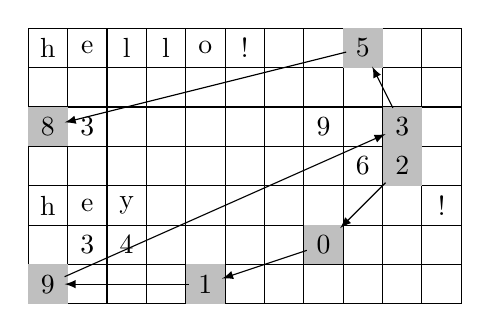
\begin{tikzpicture}[scale=0.5]
            \draw (0,0) grid (11,7);

            \draw (0.5,2.5) node{h};
            \draw (1.5,2.5) node{e};
            \draw (2.5,2.5) node{y};

            \draw (0.5,6.5) node{h};
            \draw (1.5,6.5) node{e};
            \draw (2.5,6.5) node{l};
            \draw (3.5,6.5) node{l};
            \draw (4.5,6.5) node{o};
            \draw (5.5,6.5) node{!};

            \draw (10.5,2.5) node{!};
            \draw (7.5,4.5) node{9};
            \draw (8.5,3.5) node{6};
            \draw (1.5,4.5) node{3};
            \draw (2.5,1.5) node{4};
            \draw (1.5,1.5) node{3};

            \fill[gray!50] (0,4) rectangle (1,5);
            \node (8) at (0.5,4.5) {8};
            \fill[gray!50] (8,6) rectangle (9,7);
            \node (5) at (8.5,6.5) {5};
            \fill[gray!50] (9,4) rectangle (10,5);
            \node (3) at (9.5,4.5) {3};
            \fill[gray!50] (0,0) rectangle (1,1);
            \node (9) at (0.5,0.5) {9};
            \fill[gray!50] (4,0) rectangle (5,1);
            \node (1) at (4.5,0.5) {1};
            \fill[gray!50] (7,1) rectangle (8,2);
            \node (0) at (7.5,1.5) {0};
            \fill[gray!50] (9,3) rectangle (10,4);
            \node (2) at (9.5,3.5) {2};
            \draw[<-,>=latex] (8) -- (5);
            \draw[<-,>=latex] (5) -- (3);
            \draw[<-,>=latex] (3) -- (9);
            \draw[<-,>=latex] (9) -- (1);
            \draw[<-,>=latex] (1) -- (0);
            \draw[<-,>=latex] (0) -- (2);
        \end{tikzpicture}
        \captionof{figure}{Chaque élément pointe vers le suivant.}
    \end{center}
    \note{tête de liste = dernier élément ajouté (ici 2)}
\end{frame}
\subsection{Comparaison avec un tableau}
\begin{frame}
    \frametitle{Comparaison avec un tableau}


    \begin{center}
        \begin{tabular}{cc}
            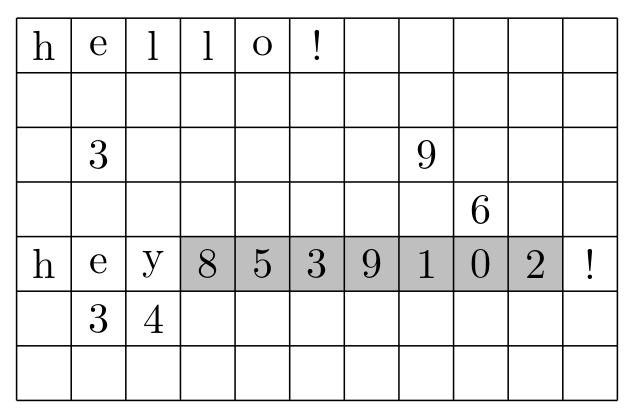
\includegraphics[width=4.5cm]{ressources/tab.png}
             &
            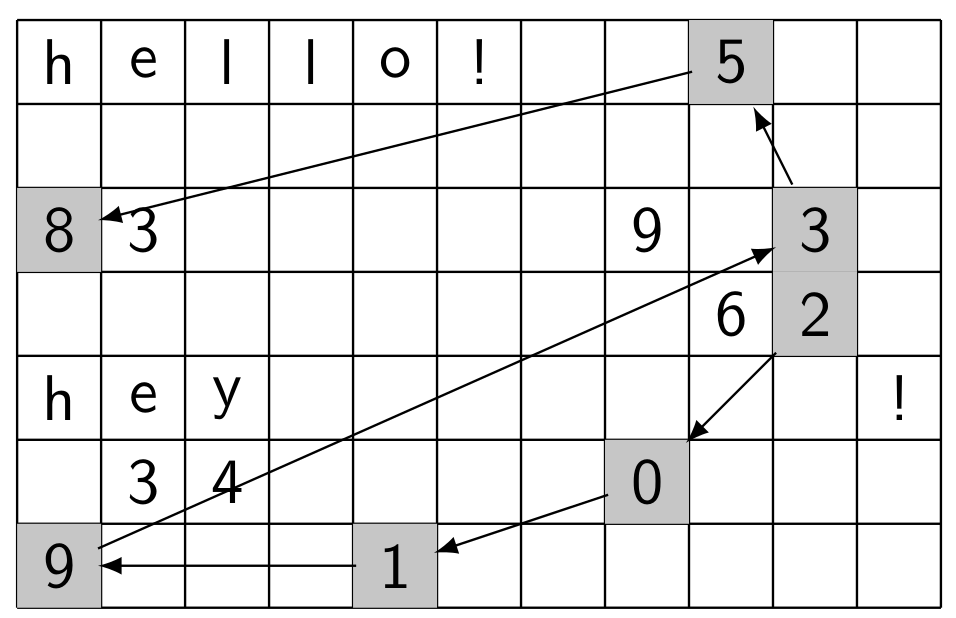
\includegraphics[width=4.5cm]{ressources/liste.png}
        \end{tabular}
    \end{center}
    \begin{activite}
        Comparer l'efficacité des deux structures lors de:
        \begin{itemize}
            \item l'ajout d'un élément,
            \item l'accès à un élément,
            \item l'insertion d'un élément.
        \end{itemize}
    \end{activite}
\end{frame}
\begin{frame}
    \frametitle{Ajouter un élément}

    \begin{center}
        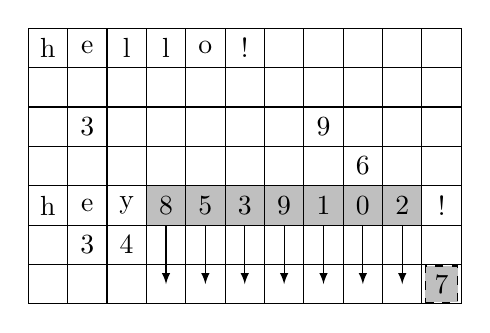
\begin{tikzpicture}[scale=0.5]
            \fill[gray!50] (3,2) rectangle (10,3);
            \draw (0,0) grid (11,7);

            \draw (0.5,2.5) node{h};
            \draw (1.5,2.5) node{e};
            \draw (2.5,2.5) node{y};

            \draw (0.5,6.5) node{h};
            \draw (1.5,6.5) node{e};
            \draw (2.5,6.5) node{l};
            \draw (3.5,6.5) node{l};
            \draw (4.5,6.5) node{o};
            \draw (5.5,6.5) node{!};

            \draw (10.5,2.5) node{!};
            \draw (7.5,4.5) node{9};
            \draw (8.5,3.5) node{6};
            \draw (1.5,4.5) node{3};
            \draw (2.5,1.5) node{4};
            \draw (1.5,1.5) node{3};

            \foreach \x/\y in {3/8,4/5,5/3,6/9,7/1,8/0,9/2}
                {\draw (\x+0.5,2.5) node{\y};
                    \draw[->,>=latex] (\x+.5,2) -- (\x+.5,.5);
                }
            \node[draw,dashed,fill=gray!50] at(10.5,.5) {7};
        \end{tikzpicture}
        \captionof{figure}{Pour ajouter 7 au tableau il faut recopier entièrement ce-dernier dans un espace libre.}
        \label{IMG}
    \end{center}
    \begin{aretenir}[]
        L'ajout d'un élément à un tableau a une complexité \textbf{linéaire} dans le pire des cas.
    \end{aretenir}
\end{frame}
\begin{frame}
    \frametitle{}

    \begin{center}
        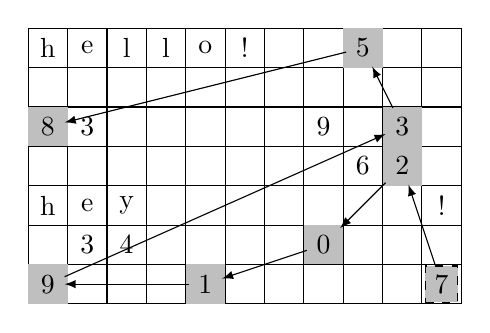
\begin{tikzpicture}[scale=0.5]
            \draw (0,0) grid (11,7);

            \draw (0.5,2.5) node{h};
            \draw (1.5,2.5) node{e};
            \draw (2.5,2.5) node{y};

            \draw (0.5,6.5) node{h};
            \draw (1.5,6.5) node{e};
            \draw (2.5,6.5) node{l};
            \draw (3.5,6.5) node{l};
            \draw (4.5,6.5) node{o};
            \draw (5.5,6.5) node{!};

            \draw (10.5,2.5) node{!};
            \draw (7.5,4.5) node{9};
            \draw (8.5,3.5) node{6};
            \draw (1.5,4.5) node{3};
            \draw (2.5,1.5) node{4};
            \draw (1.5,1.5) node{3};

            \fill[gray!50] (0,4) rectangle (1,5);
            \node (8) at (0.5,4.5) {8};
            \fill[gray!50] (8,6) rectangle (9,7);
            \node (5) at (8.5,6.5) {5};
            \fill[gray!50] (9,4) rectangle (10,5);
            \node (3) at (9.5,4.5) {3};
            \fill[gray!50] (0,0) rectangle (1,1);
            \node (9) at (0.5,0.5) {9};
            \fill[gray!50] (4,0) rectangle (5,1);
            \node (1) at (4.5,0.5) {1};
            \fill[gray!50] (7,1) rectangle (8,2);
            \node (0) at (7.5,1.5) {0};
            \fill[gray!50] (9,3) rectangle (10,4);
            \node (2) at (9.5,3.5) {2};
            \draw[<-,>=latex] (8) -- (5);
            \draw[<-,>=latex] (5) -- (3);
            \draw[<-,>=latex] (3) -- (9);
            \draw[<-,>=latex] (9) -- (1);
            \draw[<-,>=latex] (1) -- (0);
            \draw[<-,>=latex] (0) -- (2);

            \node[draw,dashed,fill=gray!50] (7) at(10.5,.5) {7};
            \draw[<-,>=latex] (2) -- (7);
        \end{tikzpicture}
        \captionof{figure}{Pour ajouter 7 à la liste, il suffit de modifier la tête de liste.}
    \end{center}
    \begin{aretenir}[]
        L'ajout d'un élément à une liste chaînée se fait en temps \textbf{constant}.
    \end{aretenir}
\end{frame}
\begin{frame}[fragile]
    \frametitle{Accéder à un élément}

    \begin{center}
        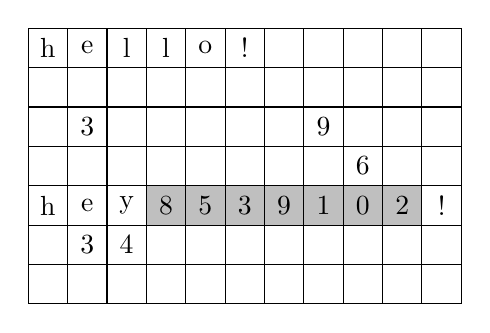
\begin{tikzpicture}[scale=0.5]
            \fill[gray!50] (3,2) rectangle (10,3);
            \draw (0,0) grid (11,7);

            \draw (0.5,2.5) node{h};
            \draw (1.5,2.5) node{e};
            \draw (2.5,2.5) node{y};

            \draw (0.5,6.5) node{h};
            \draw (1.5,6.5) node{e};
            \draw (2.5,6.5) node{l};
            \draw (3.5,6.5) node{l};
            \draw (4.5,6.5) node{o};
            \draw (5.5,6.5) node{!};

            \draw (10.5,2.5) node{!};
            \draw (7.5,4.5) node{9};
            \draw (8.5,3.5) node{6};
            \draw (1.5,4.5) node{3};
            \draw (2.5,1.5) node{4};
            \draw (1.5,1.5) node{3};

            \foreach \x/\y in {3/8,4/5,5/3,6/9,7/1,8/0,9/2}
                {\draw (\x+0.5,2.5) node{\y};}
        \end{tikzpicture}
        \captionof{figure}{Dans un tableau, l'adresse de chaque élément dépend de celle du premier.}
        \begin{lstlisting}[language=Python , basicstyle=\ttfamily\small, xleftmargin=0em, xrightmargin=0em]
adr[élément 2] = adr[élément 0] + 2×taille_élément
\end{lstlisting}
    \end{center}
    \begin{aretenir}[]
        L'accès à un élément d'un tableau se fait en temps \textbf{constant}.
    \end{aretenir}
\end{frame}
\begin{frame}
    \frametitle{}

    \begin{center}
        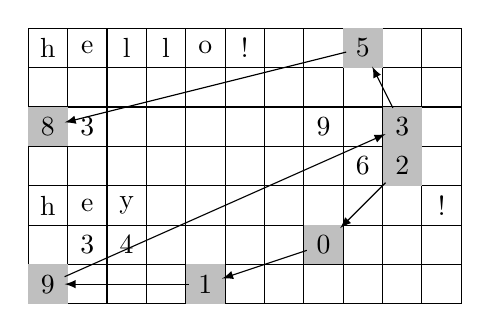
\begin{tikzpicture}[scale=0.5]
            \draw (0,0) grid (11,7);

            \draw (0.5,2.5) node{h};
            \draw (1.5,2.5) node{e};
            \draw (2.5,2.5) node{y};

            \draw (0.5,6.5) node{h};
            \draw (1.5,6.5) node{e};
            \draw (2.5,6.5) node{l};
            \draw (3.5,6.5) node{l};
            \draw (4.5,6.5) node{o};
            \draw (5.5,6.5) node{!};

            \draw (10.5,2.5) node{!};
            \draw (7.5,4.5) node{9};
            \draw (8.5,3.5) node{6};
            \draw (1.5,4.5) node{3};
            \draw (2.5,1.5) node{4};
            \draw (1.5,1.5) node{3};

            \fill[gray!50] (0,4) rectangle (1,5);
            \node (8) at (0.5,4.5) {8};
            \fill[gray!50] (8,6) rectangle (9,7);
            \node (5) at (8.5,6.5) {5};
            \fill[gray!50] (9,4) rectangle (10,5);
            \node (3) at (9.5,4.5) {3};
            \fill[gray!50] (0,0) rectangle (1,1);
            \node (9) at (0.5,0.5) {9};
            \fill[gray!50] (4,0) rectangle (5,1);
            \node (1) at (4.5,0.5) {1};
            \fill[gray!50] (7,1) rectangle (8,2);
            \node (0) at (7.5,1.5) {0};
            \fill[gray!50] (9,3) rectangle (10,4);
            \node (2) at (9.5,3.5) {2};
            \draw[<-,>=latex] (8) -- (5);
            \draw[<-,>=latex] (5) -- (3);
            \draw[<-,>=latex] (3) -- (9);
            \draw[<-,>=latex] (9) -- (1);
            \draw[<-,>=latex] (1) -- (0);
            \draw[<-,>=latex] (0) -- (2);
        \end{tikzpicture}
        \captionof{figure}{Pour accéder à l'élément de rang n il faut partir de la tête et avancer 5 fois.}
    \end{center}
    \begin{aretenir}[]
        L'accès à l'élément de rang n a une complexité \textbf{linéaire}.
    \end{aretenir}
\end{frame}
\begin{frame}
    \frametitle{Insérer un élément}

    \begin{center}
        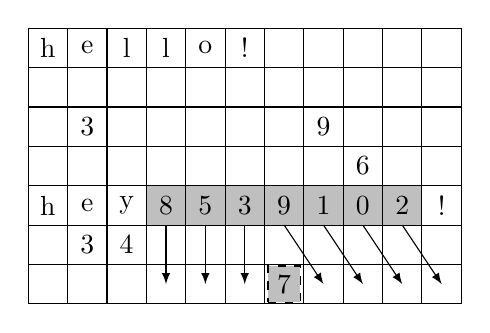
\begin{tikzpicture}[scale=0.5]
            \fill[gray!50] (3,2) rectangle (10,3);
            \draw (0,0) grid (11,7);

            \draw (0.5,2.5) node{h};
            \draw (1.5,2.5) node{e};
            \draw (2.5,2.5) node{y};

            \draw (0.5,6.5) node{h};
            \draw (1.5,6.5) node{e};
            \draw (2.5,6.5) node{l};
            \draw (3.5,6.5) node{l};
            \draw (4.5,6.5) node{o};
            \draw (5.5,6.5) node{!};

            \draw (10.5,2.5) node{!};
            \draw (7.5,4.5) node{9};
            \draw (8.5,3.5) node{6};
            \draw (1.5,4.5) node{3};
            \draw (2.5,1.5) node{4};
            \draw (1.5,1.5) node{3};

            \foreach \x/\y in {3/8,4/5,5/3,6/9,7/1,8/0,9/2}
                {\draw (\x+0.5,2.5) node{\y};
                }
            \foreach \x/\y in {3,4,5}
                {\draw[->,>=latex] (\x+.5,2) -- (\x+.5,.5);
                }
            \foreach \x/\y in {6,7,8,9}
                {\draw[->,>=latex] (\x+.5,2) -- (\x+1.5,.5);
                }
            \node[draw,dashed,fill=gray!50] at(6.5,.5) {7};
        \end{tikzpicture}
        \captionof{figure}{Pour insérer 7 dans le tableau il faut recopier entièrement ce-dernier dans un espace libre.}
        \label{IMG}
    \end{center}
    \begin{aretenir}[]
        L'insertion d'un élément dans un tableau a une complexité \textbf{linéaire} dans le pire des cas.
    \end{aretenir}

\end{frame}
\begin{frame}
    \frametitle{}

    \begin{center}
        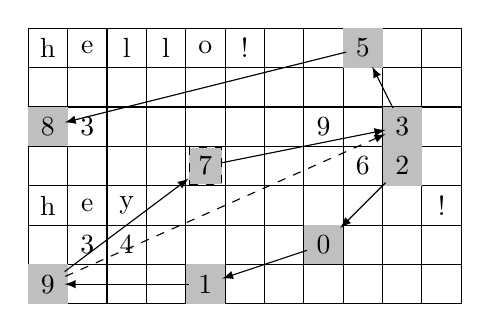
\begin{tikzpicture}[scale=0.5]
            \draw (0,0) grid (11,7);

            \draw (0.5,2.5) node{h};
            \draw (1.5,2.5) node{e};
            \draw (2.5,2.5) node{y};

            \draw (0.5,6.5) node{h};
            \draw (1.5,6.5) node{e};
            \draw (2.5,6.5) node{l};
            \draw (3.5,6.5) node{l};
            \draw (4.5,6.5) node{o};
            \draw (5.5,6.5) node{!};

            \draw (10.5,2.5) node{!};
            \draw (7.5,4.5) node{9};
            \draw (8.5,3.5) node{6};
            \draw (1.5,4.5) node{3};
            \draw (2.5,1.5) node{4};
            \draw (1.5,1.5) node{3};

            \fill[gray!50] (0,4) rectangle (1,5);
            \node (8) at (0.5,4.5) {8};
            \fill[gray!50] (8,6) rectangle (9,7);
            \node (5) at (8.5,6.5) {5};
            \fill[gray!50] (9,4) rectangle (10,5);
            \node (3) at (9.5,4.5) {3};
            \fill[gray!50] (0,0) rectangle (1,1);
            \node (9) at (0.5,0.5) {9};
            \fill[gray!50] (4,0) rectangle (5,1);
            \node (1) at (4.5,0.5) {1};
            \fill[gray!50] (7,1) rectangle (8,2);
            \node (0) at (7.5,1.5) {0};
            \fill[gray!50] (9,3) rectangle (10,4);
            \node (2) at (9.5,3.5) {2};
            \node[draw,dashed,fill=gray!50] (7) at(4.5,3.5) {7};
            \draw[<-,>=latex] (8) -- (5);
            \draw[<-,>=latex] (5) -- (3);
            \draw[<-,>=latex,dashed] (3) -- (9);
            \draw[<-,>=latex] (9) -- (1);
            \draw[<-,>=latex] (1) -- (0);
            \draw[<-,>=latex] (0) -- (2);

            \draw[->,>=latex] (7) -- (3);
            \draw[->,>=latex] (9) -- (7);
        \end{tikzpicture}
        \captionof{figure}{Pour insérer 7 au rang \emph{i} de la liste, il faut modifier le successeur de l'élément de rang \emph{i}.}
    \end{center}
    \begin{aretenir}[]
        L'insertion d'un élément à une liste chaînée se fait en temps \textbf{linéaire}.
    \end{aretenir}
\end{frame}
\begin{frame}
    \frametitle{Bilan}

    \begin{center}

        \renewcommand{\arraystretch}{2}

        \begin{tabular}{|*{3}{c|}}
            \hline
                               & \textbf{tableau} & \textbf{liste} \\
            \hline
            \textbf{ajout}     & linéaire         & constant       \\
            \hline
            \textbf{accès}     & constant         & linéaire       \\
            \hline
            \textbf{insertion} & linéaire         & linéaire       \\
            \hline
        \end{tabular}
        \renewcommand{\arraystretch}{1}

    \end{center}

\end{frame}
\section{Implémentation}
\begin{frame}[fragile]
    \frametitle{Implémentation - le maillon}

    \begin{center}
        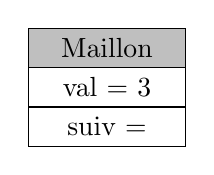
\begin{tikzpicture}
            \node[draw,fill=gray!50,minimum width=2cm, minimum height=0.5cm] (c10) at (0,1) {Maillon};
            \node[draw,minimum width=2cm, minimum height=0.5cm] (c11) at (0,.5) {val = 3};
            \node[draw,minimum width=2cm, minimum height=0.5cm] (c12) at (0,0) {suiv =};
        \end{tikzpicture}
        \captionof{figure}{Chaque maillon contient 2 informations}
    \end{center}
    \begin{center}
        \begin{lstlisting}[language=Python , basicstyle=\ttfamily\small, xleftmargin=0em, xrightmargin=0em]
class Maillon:
    """
    Crée un maillon de la liste chaînée
    """

    def __init__(self, val: int, suiv: object):
        self.valeur = val
        self.suivant = suiv
\end{lstlisting}
        \captionof{code}{Un objet \textbf{\texttt{Maillon}}}
        \label{CODE}
    \end{center}
\end{frame}
\begin{frame}
    \frametitle{La liste}
    \begin{center}
        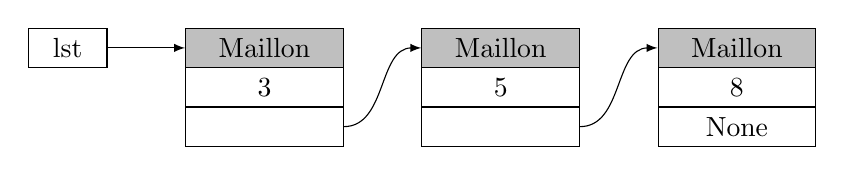
\begin{tikzpicture}[scale=.5]
            \node[draw,minimum width=1cm, minimum height=0.5cm] (lst) at (-5,2) {lst};

            \node[draw,fill=gray!50,minimum width=2cm, minimum height=0.5cm] (c10) at (0,2) {Maillon};
            \node[draw,minimum width=2cm, minimum height=0.5cm] (c11) at (0,1) {3};
            \node[draw,minimum width=2cm, minimum height=0.5cm] (c12) at (0,0) {};

            \node[draw,fill=gray!50,minimum width=2cm, minimum height=0.5cm] (c20) at (6,2) {Maillon};
            \node[draw,minimum width=2cm, minimum height=0.5cm] (c21) at (6,1) {5};
            \node[draw,minimum width=2cm, minimum height=0.5cm] (c22) at (6,0) {};

            \node[draw,fill=gray!50,minimum width=2cm, minimum height=0.5cm] (c30) at (12,2) {Maillon};
            \node[draw,minimum width=2cm, minimum height=0.5cm] (c31) at (12,1) {8};
            \node[draw,minimum width=2cm, minimum height=0.5cm] (c32) at (12,0) {None};

            \draw[->,>=latex] (lst) -- (c10);
            \draw[->,>=latex] (c12) to[out=0,in=180] (c20);
            \draw[->,>=latex] (c22) to[out=0,in=180] (c30);
        \end{tikzpicture}
        \captionof{figure}{La liste est une succession de maillons}
    \end{center}

\end{frame}
\begin{frame}[fragile]
    \frametitle{}

    \begin{center}
        \begin{lstlisting}[language=Python , basicstyle=\ttfamily\small, xleftmargin=2em, xrightmargin=1em]
lst = Maillon(3, Maillon(5, Maillon(8, None)))
\end{lstlisting}
        \captionof{code}{Chaque maillon est le suivant d'un autre.}
        \label{CODE}
    \end{center}

\end{frame}
\begin{frame}
    \frametitle{La liste - seconde approche}
    \begin{center}
        \centering
        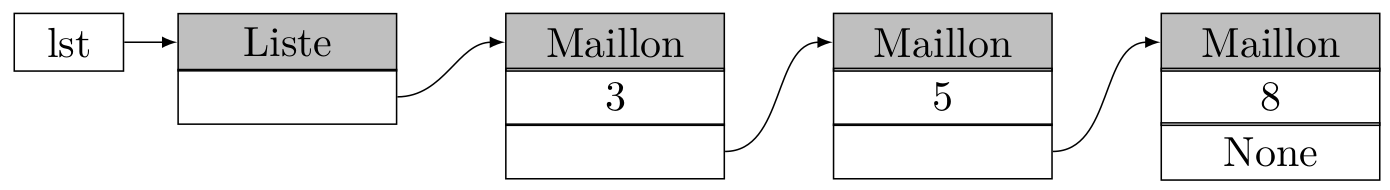
\includegraphics[width=10cm]{ressources/liste2.png}
        \captionof{figure}{L'objet \textbf{\texttt{Liste}} contient une référence à la tête.}
        \label{IMG}
    \end{center}

\end{frame}
\begin{frame}[fragile]
    \frametitle{}

    \begin{center}
        \begin{lstlisting}[language=Python , basicstyle=\ttfamily\small, xleftmargin=1em, xrightmargin=1em]
class Liste:
    """
    Crée une liste chaînée
    """

    def __init__(self):
        self.tete: Maillon = None
\end{lstlisting}
        \captionof{code}{Objet \textbf{\texttt{Liste}}}
        \label{CODE}
    \end{center}
    \note[item]{L'attribut \textit{tete} représente le premier \textit{Maillon}.}
    \note[item]{Une liste vide renvoie alors \textit{None}.}
\end{frame}
\begin{frame}
    \frametitle{}


    \begin{activite}
        \begin{enumerate}
            \item Écrire la méthode \texttt{\textbf{est\_vide(self) $\rightarrow$ bool}} qui renvoie \textbf{\texttt{True}} si la liste est vide, \textbf{\texttt{False}} sinon.
            \item Écrire la méthode \texttt{\textbf{ajoute(self, val: int) $\rightarrow$ None}} qui ajoute un \textbf{\texttt{Maillon}} en tête de la liste.
            \item Créer la liste contenant les éléments 8, 5, 3.
        \end{enumerate}
    \end{activite}

\end{frame}
\begin{frame}[fragile]
    \frametitle{}

    \begin{center}
        \begin{lstlisting}[language=Python , basicstyle=\ttfamily\small, xleftmargin=2em, xrightmargin=2em]
def est_vide(self) -> bool:
    return self.tete is None

def ajoute(self, val: int) -> None:
    self.tete = Maillon(val, self.tete)
\end{lstlisting}
    \end{center}
    \begin{center}
        \begin{lstlisting}[language=Python , basicstyle=\ttfamily\small, xleftmargin=2em, xrightmargin=2em]
lst = Liste()
lst.ajoute(8)
lst.ajoute(5)
lst.ajoute(3)
\end{lstlisting}
        \captionof{code}{Création de la liste}
        \label{CODE}
    \end{center}
\end{frame}
\begin{frame}[fragile]
    \frametitle{}

    La méthode \textbf{\texttt{\_\_str\_\_}} permettra de visualiser l'état de la liste.
\begin{center}
\begin{lstlisting}[language=Python , basicstyle=\ttfamily\small, xleftmargin=2em, xrightmargin=2em]
def __str__(self):
    m = self.tete
    s = ""
    while m is not None:
        s += str(m.valeur)+" - "
        m = m.suivant
    else:
        s += "fin"
    return s
\end{lstlisting}
\end{center}
\begin{center}
\begin{lstlisting}[language=Python , basicstyle=\ttfamily\small, xleftmargin=2em, xrightmargin=2em]
print(lst)
\end{lstlisting}
\captionof{code}{Afficher la liste}
\label{CODE}
\end{center}
\end{frame}
\section{Manipuler une liste chaînée}
\subsection{Taille de la liste}
\begin{frame}
    \frametitle{Manipuler une liste chaînée - taille}

    Pour connaître la taille de la liste il faut la parcourir entièrement.
    \begin{activite}
        \begin{enumerate}
            \item Écrire la méthode récursive \textbf{\texttt{taille\_rec(self, m: Maillon) $\rightarrow$ int}} qui renvoie la taille de la liste démarrant à \textbf{\texttt{m}}
            \item Écrire la méthode \textbf{\texttt{taille(self) $\rightarrow$ int}} qui renvoie la taille de la liste. Cette méthode utilisera \textbf{\texttt{taille\_rec}}.
            \item \textbf{Pour les plus avancés:} Écrire la méthode native (itérative) \textbf{\texttt{\_\_len\_\_(self) $\rightarrow$ int}} qui redéfinit la fonction \textbf{\texttt{len}} pour la classe \textbf{\texttt{Liste}}.
        \end{enumerate}
    \end{activite}

\end{frame}
\begin{frame}[fragile]
    \frametitle{}

    \begin{center}
        \begin{lstlisting}[language=Python , basicstyle=\ttfamily\small, xleftmargin=2em, xrightmargin=2em]
def taille_rec(self, m: Maillon) -> int:
    """
    méthode interne pour calculer la taille de la chaîne
    """
    if m is None:
        return 0
    else:
        return 1 + self.taille_rec(m.suivant)
\end{lstlisting}
    \end{center}

\end{frame}
\begin{frame}[fragile]
    \frametitle{}

    \begin{center}
        \begin{lstlisting}[language=Python , basicstyle=\ttfamily\small, xleftmargin=2em, xrightmargin=2em]
def taille(self) -> int:
    """
    appel principal de la méthode récursive pour mesurer
    la taille de la chaîne
    """
    return self.taille_rec(self.tete)
\end{lstlisting}
    \end{center}
    \begin{center}
        \begin{lstlisting}[language=Python , basicstyle=\ttfamily\small, xleftmargin=2em, xrightmargin=2em]
print(lst.taille())
\end{lstlisting}
        \captionof{code}{Affichage de la taille de la liste}
        \label{CODE}
    \end{center}
\end{frame}
\begin{frame}[fragile]
    \frametitle{}

    \begin{center}
        \begin{lstlisting}[language=Python , basicstyle=\ttfamily\small, xleftmargin=2em, xrightmargin=2em]
def __len__(self) -> int:
    maillon = self.tete
    taille = 0
    while maillon is not None:
        maillon = maillon.suivant
        taille += 1
    return taille
\end{lstlisting}
    \end{center}
    \begin{center}
        \begin{lstlisting}[language=Python , basicstyle=\ttfamily\small, xleftmargin=2em, xrightmargin=2em]
print(len(lst))
\end{lstlisting}
        \captionof{code}{Appel de la fonction \textbf{\texttt{len}}}
        \label{CODE}
    \end{center}
\end{frame}
\subsection{N-ième élément}
\begin{frame}
    \frametitle{N-ième élément}

    Il faut parcourir la liste jusqu'au rang \emph{n} pour trouver l'élément.
    \begin{activite}
        \begin{enumerate}
            \item Écrire la méthode récursive \textbf{\texttt{get\_element\_rec(self, n: int m: Maillon) $\rightarrow$ int}} qui renvoie la valeur du n-iéme élément de la liste démarrant à \textbf{\texttt{m}}
            \item Écrire la méthode \textbf{\texttt{get\_element(self) $\rightarrow$ int}} qui renvoie la valeur du n-iéme élément. Cette méthode utilisera \textbf{\texttt{get\_element\_rec}}.
            \item \textbf{Pour les plus avancés:} Écrire la méthode native (itérative) \textbf{\texttt{\_\_getitem\_\_(self) $\rightarrow$ int}} qui redéfinit la structure à crochets (\textbf{\texttt{lst[n]}}) pour la classe \textbf{\texttt{Liste}}.
        \end{enumerate}
    \end{activite}

\end{frame}
\begin{frame}[fragile]
    \frametitle{Correction}

    \begin{center}
    \begin{lstlisting}[language=Python , basicstyle=\ttfamily\small, xleftmargin=0em, xrightmargin=0em]
def get_element_rec(self, n: int, m: Maillon) -> int:
    """
    méthode interne pour renvoyer le n-ième élément.
    """
    if n == 0:
        return m.valeur
    else:
        return self.get_element_rec(n-1, m.suivant)
\end{lstlisting}
    \end{center}

\end{frame}
\begin{frame}[fragile]
    \frametitle{Correction}

    \begin{center}
    \begin{lstlisting}[language=Python , basicstyle=\ttfamily\small, xleftmargin=0em, xrightmargin=0em]
def get_element_rec(self, n: int, m: Maillon) -> int:
    """
    méthode interne pour renvoyer le n-ième élément.
    """
    # n est plus grand que la taille de la liste
    if m is None:
        raise IndexError("indice invalide")
    if n == 0:
        return m.valeur
    else:
        return self.get_element_rec(n-1, m.suivant)
\end{lstlisting}
    \captionof{code}{Avec gestion du dépassement de taille}
    \label{CODE}
    \end{center}

\end{frame}
\begin{frame}[fragile]
    \frametitle{Correction}

    \begin{center}
    \begin{lstlisting}[language=Python , basicstyle=\ttfamily\small, xleftmargin=1em, xrightmargin=1em]
def get_element(self, n: int) -> int:
    """
    appel principal de la méthode récursive pour renvoyer le n-ième élément
    """
    return self.get_element_rec(n, self.tete)
\end{lstlisting}
    \end{center}
    \begin{center}
        \begin{lstlisting}[language=Python , basicstyle=\ttfamily\small, xleftmargin=2em, xrightmargin=2em]
print(lst.get_element(3))
\end{lstlisting}
        \captionof{code}{Appel de la fonction}
        \label{CODE}
    \end{center}
\end{frame}
\begin{frame}[fragile]
    \begin{center}
    \begin{lstlisting}[language=Python , basicstyle=\ttfamily\small, xleftmargin=2em, xrightmargin=2em]
def __getitem__(self, n: int) -> int:
    """
    renvoie l'élément de rang n. Les indices commencent à 0.
    """
    maillon = self.tete
    i = 0
    while i < n and maillon is not None:
        maillon = maillon.suivant
        i += 1

    if maillon is None:
        raise IndexError("indice invalide")

    return maillon.valeur
\end{lstlisting}
    \end{center}
    \begin{center}
        \begin{lstlisting}[language=Python , basicstyle=\ttfamily\small, xleftmargin=2em, xrightmargin=2em]
print(lst[3])
\end{lstlisting}
        \captionof{code}{Appel de la fonction}
        \label{CODE}
    \end{center}
\end{frame}
\subsection{Insertion}
\begin{frame}
    \frametitle{Insertion}

L'insertion d'un élément au rang \emph{n} peut être réalisée sur le même principe. On prendra le parti d'insérer l'élément en fin si la valeur de \emph{n} dépasse la taille de la liste.


    \begin{center}
        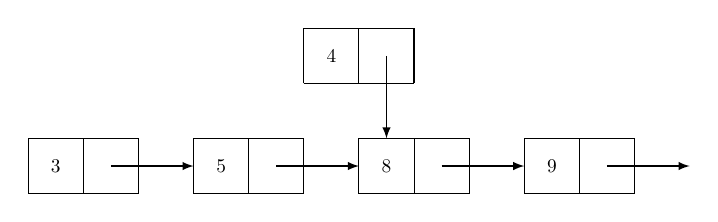
\begin{tikzpicture}[scale=0.7, transform shape]
            \foreach \x/\y in {0/3,3/5,6/8,9/9}{
            \draw (0+\x,0) grid (2+\x,1);
            \node at (.5+\x,.5) {\y};
            \draw[->,>=latex] (1.5+\x,.5) -- (3+\x,.5);
            }
            \draw (5,2) grid (7,3);
            \node at (5.5,2.5) {4};
            \draw[->,>=latex] (6.5,2.5) -- (6.5,1);
        \end{tikzpicture}
        \captionof{figure}{Insertion de 4 au rang 2}
    \end{center}
    \begin{center}
        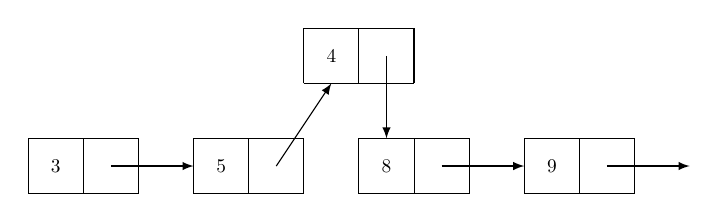
\begin{tikzpicture}[scale=0.7, transform shape]
            \foreach \x/\y in {0/3,3/5,6/8,9/9}{
            \draw (0+\x,0) grid (2+\x,1);
            \node at (.5+\x,.5) {\y};
            }
            \foreach \x/\y in {0/3}{
            \draw[->,>=latex] (1.5+\x,.5) -- (3+\x,.5);
            }
            \foreach \x/\y in {6/8,9/9}{
            \draw[->,>=latex] (1.5+\x,.5) -- (3+\x,.5);
            }
            \draw (5,2) grid (7,3);
            \node at (5.5,2.5) {4};
            \draw[->,>=latex] (6.5,2.5) -- (6.5,1);
            \draw[->,>=latex] (4.5,.5) -- (5.5,2);
        \end{tikzpicture}
        \captionof{figure}{Seconde étape}
    \end{center}
\end{frame}
\begin{frame}
    \frametitle{}

\begin{activite}
\begin{enumerate}
    \item Écrire la fonction récursive \textbf{\texttt{inserer\_rec(self, val: int, n: int, m: object) $\rightarrow$ None}} qui insère l'élément au rang \textbf{\texttt{n}}.
    \item Écrire la fonction \textbf{\texttt{inserer(self, val: int, n: int) $\rightarrow$ None}} qui insère l'élément \textbf{\texttt{val}} au rang \textbf{\texttt{n}}. Cette fonction gérera le cas ou \textbf{\texttt{n = 0}}.
\end{enumerate}
\end{activite}
\begin{aretenir}[Remarque]
Il faut remarquer que la fonction \textbf{\texttt{inserer\_rec}} place en réalité l'élément au rang \textbf{\texttt{n+1}}.
\end{aretenir}
\end{frame}
\begin{frame}[fragile]
    \frametitle{Correction}

\begin{center}
\begin{lstlisting}[language=Python , basicstyle=\ttfamily\small, xleftmargin=2em, xrightmargin=2em]
def inserer_rec(self, val: int, n: int, m: object) -> None:
    """
    méthode interne pour placer val au rang n
    si n est trop grand, place l'élément en fin de liste
    """
    if m.suivant is None or n == 0:
        nouveau = Maillon(val, m.suivant)
        m.suivant = nouveau
    else:
        self.inserer_rec(val, n-1, m.suivant)
\end{lstlisting}
\end{center}

\end{frame}
\begin{frame}[fragile]
    \frametitle{}

\begin{center}
\begin{lstlisting}[language=Python , basicstyle=\ttfamily\small, xleftmargin=2em, xrightmargin=2em]
def inserer(self, val: int, n: int) -> None:
    """
    appel principal de l'insertion pour placer val en n
    """
    # gestion du cas particulier où l'insertion est en début
    if n == 0:
        nouveau = Maillon(val, self.tete)
        self.tete = nouveau
    else:
        # n-1 pour ajuster la position
        self.inserer_rec(val, n-1, self.tete)
\end{lstlisting}
\end{center}

\end{frame}
\end{document}